\documentclass[11pt]{article}

\usepackage[hyphens]{url}

\usepackage{hyperref}
\hypersetup
{
    breaklinks = true,
    allcolors = black,
    linktoc = all
}

\usepackage{graphicx}

\usepackage{multicol}
\setlength{\columnseprule}{0.4pt}

\usepackage{listings}

\usepackage[english]{babel}
\usepackage[utf8]{inputenc}
\usepackage{fancyhdr}
\pagestyle{fancy}
\fancyhf{}
\rhead{James Burton}
\lhead{ID: 4251529}
\fancyfoot[C]{\thepage}

\usepackage{titling}
\title
{ 
    \vspace{10em}
    G53IDS - Interim Report \\
    \hfill \break
    \large Embedded Domain Specific Language for \\
    Describing Recipes in Haskell
}

\setlength{\droptitle}{-10em}

\author{James Burton - 4251529 - psyjb6}

\begin{document}
    \maketitle
    \newpage

    \tableofcontents
    \newpage

    \section{Introduction}
    Consider the following recipe to make a cup of tea:

    \begin{tt}
    \small
    \begin{lstlisting}
    - Boil some water
    - Pour over a teabag
    - Wait for 3 minutes
    - Remove the teabag
    - Add milk (optional)
    \end{lstlisting}
    \end{tt}

    This is a very simple but useful recipe that many people
    will perform, in some cases, many times a day over their lives.
    What we can realise by looking at this recipe is that it actually
    consists of many smaller recipes, such as boiling water and
    combining tea with milk, performed in a certain order. This
    raises the question, to what extent does the order matter and
    to what extent can we rearrange things in order to make the recipe
    more efficient? No doubt you have done this, maybe subconsciously,
    while cooking at home. Furthermore which steps can be done
    concurrently in the event that multiple people are cooking e.g.
    in a professional kitchen with a full brigade? \\

    Perhaps closer to computer science, we could also ask, how could
    we instruct a robot to do this? After doing some research on
    robotic chefs it appears that not a huge number exist.
    There is one home cooking robot \cite{robot} which uses motion
    capture in order to learn recipes. In my opinion this is rather
    restrictive. It presumes that the human performs the recipe in
    the optimal manner and it would be very difficult to model
    a brigade system in this way. In reality there is a limited set
    of fundamental actions that one becomes able to perform when
    learning to cook. Recipes can then be performed using a sequence
    of these actions. Representing recipes like this would allow us
    to take a robot programmed to perform each of the fundamental
    actions and tell it how to cook literally anything. This is the
    same principle as taking code written in a high level language
    and compiling it down into a sequence of low level actions in
    assembly language. \\

    So we've established that if we can structure recipes in a more
    formal way then we will have a great amount of freedom in terms
    of how we process them whether it be optimisation for a human
    chef or full on automation. My contributions / planned contributions
    to this are the following:

    \begin{itemize}
        \item Define a set of combinators as an EDSL in Haskell and show that
        they can be used to describe a wide variety of recipes (Section 2).

        \item The combinators describe a recipe but we then need to know
        how to execute a recipe as a sequence of the fundamental actions
        mentioned above. Fortunately, as described above, recipes are just
        a combination of simpler recipes meaning that we can recursively
        define the actions necessary to perform complex recipes as long
        as we have manually defined which action are required for each
        combinator (Section 3).

        \item We now have a way to describe recipes and a way to show the
        sequence of actions to complete a recipe but now we need to apply
        them to something. Using the operational semantics of recipes
        we can optimise and schedule recipes for a given kitchen system.
        We can then express this in several ways including printing steps,
        drawing the cooking process as a graph or simulating the recipe
        within the given kitchen setup (Section 4).
    \end{itemize}

    \section{Describing Recipes}
    In this section I shall outline the EDSL for describing recipes.
    The EDSL is implemented in the functional programming language
    called Haskell which has been used for many EDSLs in the past \cite{hudak}.
    Michael Snoyman, creator of Yesod (a Haskell Web Framework), stated
    many advantages of using Haskell for EDSLs among which were that
    the type system helps catch mistakes and Haskell allows us to
    overload almost any syntax \cite{snoyman}.

    \subsection{A Cup of Tea}
    Consider our cup of tea example from earlier. We can start by
    defining all of our ingredients:

    \begin{tt}
    \small
    \begin{lstlisting}
        milk, teabag, water :: Recipe
        milk = Ingredient "milk"
        teabag = Ingredient "teabag"
        water = Ingredient "water"
    \end{lstlisting}
    \end{tt}

    The next step is to start describing what we want to transform
    those ingredients into for example:

    \begin{tt}
    \small
    \begin{lstlisting}
        boilingWater, blackTea :: Recipe
        boilingWater = heat 100 water
        blackTea = (teabag >< boilingWater) >>> Wait 5
    \end{lstlisting}
    \end{tt}

    We've introduced three things here. \texttt{heat} is simply
    a function meaning heat the given recipe to the given temperature.
    \texttt{><} is our combine operator and simply means mix the
    given recipes together. Finally \texttt{>>>} is our sequencing
    operator meaning do the first recipe then the second. The types
    for these are as follows: 
    
    \begin{tt}
    \small
    \begin{lstlisting}
        heat :: Temperature -> Recipe -> Recipe
        (><) :: Recipe -> Recipe -> Recipe
        (>>>) :: Recipe -> Recipe -> Recipe
    \end{lstlisting}
    \end{tt}

    We can now use the above to define our cup of tea recipe as follows:

    \begin{tt}
    \small
    \begin{lstlisting}
        cupOfTea :: Recipe
        cupOfTea = blackTea >< milk
    \end{lstlisting}
    \end{tt}

    Now you may notice that we haven't mentioned preparation of ingredients,
    for example measuring how much of them to use. While experimenting with
    the basic representation of a recipe and the different ways to interpret
    it we thought it would be beneficial to keep the combinators as simple
    and abstract as possible. This means that, for now, we will be describing
    recipes "cooking show" style where we presume everything is conveniently
    measured and prepared in a bowl next to the chef.

    \subsection{Currying - But Not What You Think}
    In this section I shall introduce the full set of combinators we are
    currently working with and proceed to build up a more complex recipe.

    \begin{figure}[ht]
        \centering
            \begin{multicols}{2}
                \raggedright
                \footnotesize
                \texttt{ingredient :: String -> Recipe} \\
                The recipe \texttt{(ingredient s)} simply represents an ingredient
                with the name s.

                \texttt{heat :: Temperature -> Recipe -> Recipe} \\
                \texttt{heat t r} means to heat the recipe r to the temperature t.

                \texttt{wait :: Time -> Recipe} \\
                \texttt{wait t} simply means do nothing for t amount of time.
                The decision to for \texttt{wait} to not include a recipe as
                an argument was very deliberate and will be discussed later
                in this subsection.

                \texttt{(><) :: Recipe -> Recipe -> Recipe} \\
                The recipe \texttt{r1 >< r2} is the combination of r1 and r2.
                The details of the method you use to combine the recipes are
                not yet captured.

                \texttt{(>>>) :: Recipe -> Recipe -> Recipe} \\
                \texttt{r1 >>> r2} represents the sequence of r1 and r2 i.e.
                perform recipe r1 followed by recipe r2.
            \end{multicols}
        \caption{Combinators for defining recipes}
    \end{figure}

    For the sake of conciseness I shalln't bother listing all the ingredient
    declarations here as they are relatively straightforward. \\

    We could just create a complex recipe outright however, this would be rather
    verbose and is likely to repeat a lot of code which somewhat goes against
    the core principles of DSLs and Haskell. Therefore we shall begin by defining
    some extra combinators made from our fundamental combinators. \\

    Marinating is a frequently used recipe so let's write a function for it:
    \begin{tt}
    \small
    \begin{lstlisting}
    marinate :: Recipe -> [Recipe] -> Recipe
    marinate r' []     = r'
    marinate r' [r]    = r' >< r
    marinate r' (r:rs) = marinate r' (foldr (><) r rs)
    \end{lstlisting}
    \end{tt}
    \texttt{marinate r' rs} means marinate \texttt{r'} in a marinade composed
    of the list of recipes \texttt{rs}. \\

    Due to the compositional nature of our combinators it is easy to create new
    ones like \texttt{marinate} thus allowing us to avoid repeating common
    sequences of recipes. There is no need to adjust any of our functions that
    work on recipes to work with \texttt{marinate} because it's just a combination
    of the combinators we already support. \\

    A huge number of recipes start by heating olive oil in a pan then adding something.
    We define the following combinator for this:
    \begin{tt}
    \small
    \begin{lstlisting}
    preheatOil :: Temperature -> Recipe -> Recipe
    preheatOil t r = oil >< r
        where oil = heat t oliveOil
    \end{lstlisting}
    \end{tt}
    That is \texttt{preheatOil Medium onion} means heat some olive oil on medium heat
    then add some onion. \\

    I'm now going to explain the reasoning behind \texttt{wait} not taking a recipe as
    an argument. What this allows us to do is use \texttt{wait} in multiple ways.
    \texttt{wait t >< r} means perform recipe r for t amount of time whereas
    \texttt{r >>> wait t} means perform recipe r then wait for t. Using this we
    can define another combinator to allow us to heat a recipe at a given temperature
    but also for a certain time:
    \begin{tt}
    \small
    \begin{lstlisting}
    heatFor :: Temperature -> Recipe -> Time -> Recipe
    heatFor temp r time = (heat temp r) >< (wait time)
    \end{lstlisting}
    \end{tt}

    So let's get to that more complex recipe I mentioned earlier, Chicken Jalfrezi!
    \begin{tt}
    \small
    \begin{lstlisting}
    spicedChicken :: Recipe
    spicedChicken = marinate chicken
        [cumin, coriander, turmeric]

    chickenAndPeppers :: Recipe
    chickenAndPeppers = heatFor Medium
        (cookedChicken >< redPeppers) 10
        where cookedChicken = heatFor Medium
                              spicedChicken 10

    jalfreziSauce :: Recipe
    jalfreziSauce = heatFor Medium
                    (sauceBase >< spices) 10
        where
            onionMix     = onion >< garlic
                        >< greenChilli
            cookedOnions = heatFor Medium
                           (preheatOil Medium onionMix) 5
            spices       = cumin >< coriander
                           >< turmeric >< garamMasala
            sauceBase    = cookedOnions >< water
                           >< tinnedTomatoes >< spices

    chickenJalfrezi :: Recipe
    chickenJalfrezi = heatFor Medium chickenJalfrezi' 5
        where chickenJalfrezi' = chickenAndPeppers
                                 >< jalfreziSauce
                                 >< cherryTomatoes
    \end{lstlisting}
    \end{tt}
    And there we have it. Quite a large recipe expressed formally with
    multiple reusable components. As the project continues, the set of
    combinators will continue to evolve as we run in to issues. Some of
    these issues have already been discovered and will be discussed later
    (Section 3.3).

    \subsection{Conditionals}

    Many recipes have some sort of condition attached to them which dictate
    whether or not they are completed.This could be reaching a certain
    temperature or a certain amount of time elapsing. This functionality
    is not currently captured by our combinators so we need to introduce
    the concept of a conditional recipe. The current plan is to implement
    another constructor:

    \begin{tt}
    \small
    \begin{lstlisting}
    forall a. Eq a => Recipe `Until` a
    \end{lstlisting}
    \end{tt}

    That is for any type that supports equality, allow us to use it as a
    condition for our recipe so \texttt{r `Until` c} would mean "perform
    recipe r until conditon c evaluates to true".

    \subsection{Moving Forward}
    At the time of writing this interim report, the combinators we
    have are decent but not perfect. There are several crucial pieces
    of information not captured such as measurements and, as mentioned
    above, conditionals and optional recipes are not yet implemented. \\

    As the project continues we will naturally be provided with an
    opportunity to scrutinise the set of combinators we are working
    with by analysing any issues we run into. \\

    \section{Meaning of a Recipe}

    Our set of combinators allow us to describe a recipe, but what does
    a recipe actually mean? What are the different ways it can be
    interpreted? In this section we will discuss these possible interpretations.
    
    \subsection{Ingredient Analysis}

    The end result of all recipes is just the result of transforming and combining
    the initial ingredients in some way. Extracting a list of ingredients from
    one of our recipes would be really simple as \texttt{Ingredient} is it's own
    constructor in our recipe type. Once we have this list we can process it in
    a variety of ways. \\
    
    One such interpretation could be to evaluate the cost of the recipe and create
    a shopping list of sorts. Even the cost of a recipe has multiple interpretations.
    For example the recipe may only use 50g of flour however, if we don't already have
    some flour then we would have to buy an entire bag so we may wish to use that cost
    instead. \\

    If we had access to some sort of database with details about ingredients we could
    work out the nutritional values of a recipe, which diets it supports and the range
    of flavours present in the dish. This could then possibly be used to recommend
    susbstitutes to meet certain requirements or, going back to our shopping list idea,
    in the event that an item is out of stock. \\

    \subsection{Executing a Recipe}

    How do we actually perform a recipe? We need to translate our declarative
    recipe into a set of actions. Again if we can make these compositional
    then we will only need to change our definition in the event of a
    new fundamental combinator. \\
    
    If we consider our description of a recipe as a tree then the actions
    we can choose to complete first are the leaves of the tree. This means
    that we have a set of actions that we can possibly perform at any given
    time and this set of actions becomes smaller as we move to the root of
    the tree i.e. as time progresses. \\

    \begin{figure}[ht]
        \centering
            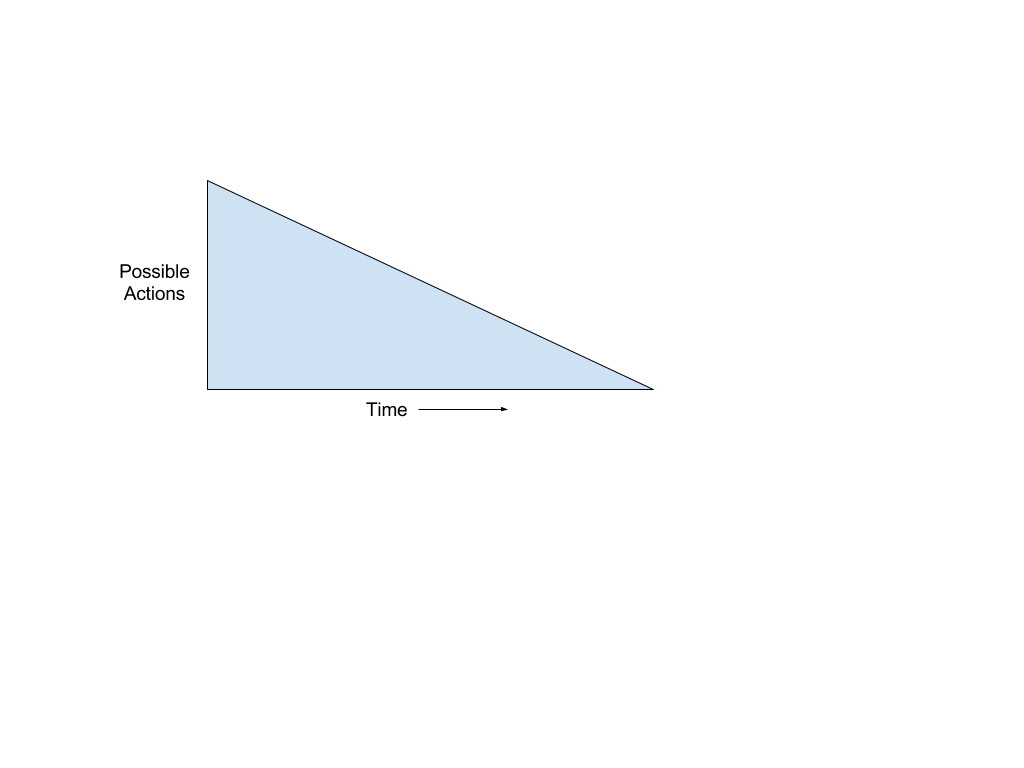
\includegraphics[width=7cm,keepaspectratio]{actions_time.png}
        \caption{Number of possible actions over time.}
    \end{figure}
    
    We can model this relationship by translating our description of a recipe into a recipe process.
    A recipe process is a mapping of time to a recipe action \texttt{RP = Time -> RA}.
    A recipe action is a list of the possible actions you could be doing,
    \texttt{RA = [Action]}, actions being fundamental things such as getting
    an ingredient or stirring something. At this point a full set of actions
    has not been created but here are some initial thoughts:

    \begin{tt}
    \small
    \begin{lstlisting}
    data Action =
        Get Recipe
        -- Heat
        | Preheat Int
        | Refrigerate Recipe
        | PlaceInHeat Recipe
        | LeaveRoomTemp Recipe
        | Freeze Recipe
        -- Wait
        | DoNothing
        -- Combine
        | PlaceAbove Recipe Recipe
        | PlaceIn Recipe Recipe
        | PourOver Recipe Recipe
        | Mix Recipe Recipe
        deriving Show
    \end{lstlisting}
    \end{tt}

    While a recipe action is described as a list of recipes above. It may turn out that some
    sort of tree structure is more appropriate.

    \subsection{Some Issues}

    While writing the function to translate a recipe into a tree of actions it became apparent
    that there were some issues with the fundamental combinators. Consider the following
    recipe \texttt{(r1 >< r2) >>> (r3 >< r4)}, that is "combine r1 and r2" then "combine r3 and r4".
    This would translate into the following tree of actions:

    \begin{figure}[ht]
        \centering
            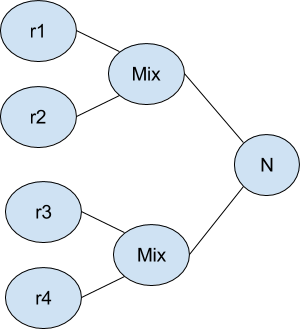
\includegraphics[width=5cm,keepaspectratio]{issue1.png}
        \caption{Action tree for the above recipe.}
    \end{figure}

    The issue is, what should the action at node N be? The cause of this issue is
    that we have added meaning to a recipe that doesn't exist in the form of the sequencing
    operator. This contradicts the statement that "a DSL should capture the semantics of the
    domain and nothing more" \cite{hudak}. Sequencing of steps only matters in a recipe if
    the steps interact with each other. This is automatically captured by the tree like nature
    of our combinators. What has happened in this recipe is we have tried to enforce sequencing
    on two unrelated recipes. \\

    One could argue that this is an issue that should be ruled out by a type checker. As SPJ
    said "we can’t expect abstract syntax to rule out all bag programs, that’s what type
    checkers are for" \cite{core}. On the other hand I would argue that what is being talked
    about here is the prevention of programs that make no sense for example subtracting an integer
    from a string. In our case the recipe should make sense and as mentioned there is evidence
    of a more fundamental issue with the DSL design therefore it makes sense to directly address
    and fix this issue. \\
    
    It may seem as though we can just remove the sequencing combinator to fix this issue however,
    sequencing or combining our wait combinator with a recipe is our way of determining the
    difference between "do r then wait" and "do r for x amount of time". This highlights another
    issue which is that our combine combinator has too many purposes. In the presentation that
    accompanied the financial contracts language it was stated that combinators should have
    one responsibility \cite{contracts-pp}. Our solution is to provide this functionality 
    with our concept of conditional recipes (Section 2.3). \\

    \section{Concrete Implementation}

    If we want to have an effective method of scheduling / optimising these actions then it would
    be useful to know more about the environment in which they are being performed. We will do this
    by providing a model in the form of a kitchen data type that can be used to store relevant
    information. Overall the structure of the project is now looking something like the following:
    
    \begin{figure}[ht]
        \centering
            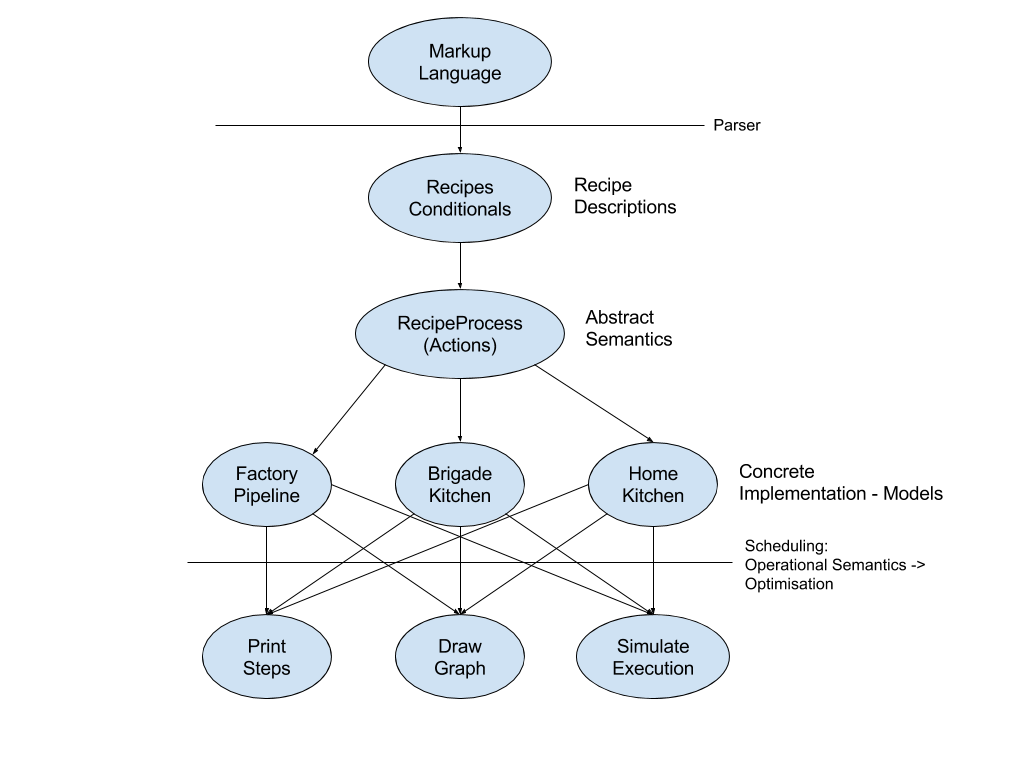
\includegraphics[width=\textwidth,keepaspectratio]{recipe_flow.png}
        \caption{Components of the recipe system.}
    \end{figure}

    \subsection{Kitchens}

    In a home kitchen we only have a small set of "paths of execution", which we'll refer to as stations,
    "stations" for example one oven, one human etc. Each of these stations is only capable of performing
    certain actions. The oven can only heat something whereas the human has to put that thing into the oven.
    In a brigade system we would have many stations each responsible for various things. The kitchen data
    type will also need to contain functions to call in order to get any relevant information to be used
    in our conditionals such as the current temperature of an oven or the current time. At this point in
    the project this data type has not been designed except for the basic concept as just detailed.

    \subsection{Optimisations, Graphs and Simulations}

    So we've described a recipe in a declarative sense, compiled it into a set of actions and modelled
    the environment in which we're cooking. Now we can start looking at how to process and display this
    information in a useful way to the user. The first would be to optimise the recipe and schedule it.
    By this we mean trying to perform as many tasks concurrently as possible. We could also run through
    the process of this schedule either in the form of a simulation or actually controlling some automated
    system. It may also be sufficient to just print out the schedule either as a list of steps for each
    station or displayed as a tree / graph of some sort.

    \section{Progress}

    This section focuses on the schedule of the project and the progress made so far.
    
    \subsection{Project Management}

    The original project plan that was submitted with the project proposal is included below:

    \begin{enumerate}
        
        \item Create project proposal and email to supervisor
        (deadline 13th October).

        \item Submit completed ethics clearance form to supervisor
        (deadline 23rd October).

        \item Amend project proposal based on feedback from
        supervisor and submit amended version (deadline 23rd October).

        \item Read \cite{hudak, contracts, pretty} to gain a better
        understanding of the DSL design process.

        \item Boil down, if you'll forgive the pun, a few recipes
        into their components and recreate the recipes in terms
        of a set of combinators. Try to create other more complex
        recipes and repeat until a satisfactory set of combinators
        is found.

        \item Define algebraic properties of the combinators.

        \item Consider various representations of recipes and the
        combinators e.g. as functions or as data structures.

        \item Write and submit interim report (deadline 8th December).

        \item Mainly revise for other modules over Christmas and during
        exams.

        \item Once the core components of the DSL are in place
        consider specifics such as temperature being centigrade,
        farenheit or gas mark.

        \item Create system to output recipes from the DSL into a format
        similar to that of a regular recipe.

        \item Create parser to read recipe formatted text into the DSL.

        \item Experiment with various applications of the DSL such
        as finding steps that can be executed concurrently.

        \item Outline contents for final report.

        \item Write and submit final report (deadline 24th April).

    \end{enumerate}

    \begin{figure}[ht]
        \centering
            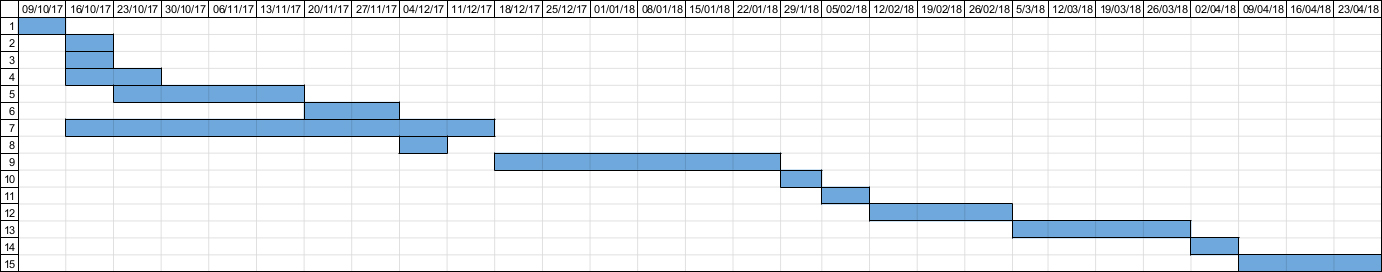
\includegraphics[width=\textwidth,keepaspectratio]{gantt_chart.jpg}
        \caption{Project plan gantt chart from the project proposal.}
    \end{figure}

    There has been some adjustment to the original project schedule. Initially I thought that I would spend
    the first half of the project designing the combinators from Section 2.2 however, my supervisor suggested
    it would be better to quickly define an initial set of combinators then use them to design and develop the
    rest of the project. This was in order to prevent being stuck refining the combinators forever and not having
    anything else to show. Refining the combinators while developing other sections is also useful because issues
    can often be brought to light that would otherwise have gone unnoticed. \\

    Below is an updated plan for the remainder of the project:

    \begin{enumerate}

        \item Continue to refine and adjust the set of combinators and set of
        actions as other areas of the project are developed.

        \item Finish implementation of denotational semantics and recipe processes.

        \item Catch up on other coursework.

        \item Mainly revise for other modules over Christmas and during
        exams.

        \item Create kitchen data type for concrete implementation.

        \item Create systems to print recipes in a variety of ways.

        \item Define operational semantics to see if any optimisations are possible
        then work on the scheduling of a recipe.

        \item Once the core components of the DSL are in place
        consider specifics such as units of temperature and allowing the
        measuring of ingredients / recipes.

        \item Outline contents for final report.

        \item Write and submit final report (deadline 24th April).

    \end{enumerate}

    \begin{figure}[ht]
        \centering
            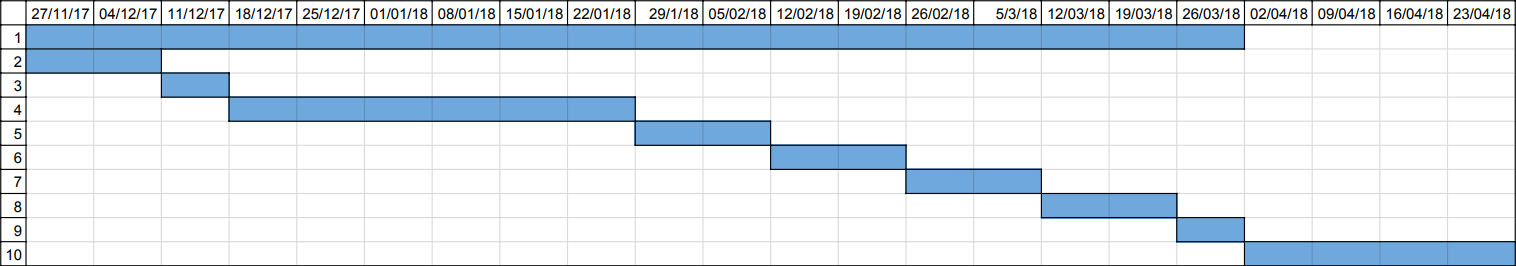
\includegraphics[width=\textwidth,keepaspectratio]{gantt_chart2.jpg}
        \caption{Updated project plan gantt chart.}
    \end{figure}

    \subsection{Contributions and Reflections}

    Currently the project is progressing well. While certain areas such as the concrete implementation have
    not been developed or fully designed yet, there is at least a firm idea of the direction the project will go
    over the remainder of its duration. The scrum development methodology seems to be effective in allowing
    flexibility. For example quite a bit of time was spent thinking of how to represent the semantics of a
    recipe and I am now in the process of implementing that system. \\
    
    As far as I am aware there is no exsiting EDSL for describing recipes or manipulating recipes. While DSLs
    and various forms of semantics are certainly not new, exactly how to apply them to recipes is relatively
    unexplored. The contributions made so far are as follows:

    \begin{itemize}
        \item A small set of combinators that can be used to describe a wide variety of recipes.

        \item A partial implementation of recipe processes which detail how to actually perform a recipe.

        \item A plan to model kitchens as a set of stations in order to schedule or simulate a recipe
        in a certain environment.
    \end{itemize}

    These will be further developed and expanded on over the remainder of the project.

    \section{Related Work}

    As stated in the previous section, a recipe DSL is something that has not been done before.
    However, the various componenets such as the concept of a DSL have been around for a long time.
    A DSL that has some similarities to the recipe DSL is that for financial contracts \cite{contracts}.
    Reading that paper provided a lot of inspiration and guidance regarding how to break down recipes
    and proceed with the design of the language. There has also been research done into DSLs
    in general for example \cite{hudak} and \cite{snoyman}.

    \newpage
    \begin{thebibliography}{5}

        \bibitem{robot}
        The Guardian. 2015. \textit{Future of food: how we cook}.
        \url{https://www.theguardian.com/technology/2015/sep/13/future-of-food-how-we-cook}

        \bibitem{hudak}
        Paul Hudak. Domain Specific Languages. Department of Computer
        Science, Yale University, December 15, 1997.

        \bibitem{snoyman}
        Michael Snoynman. O'Reilly Webcast: Designing Domain Specific
        Languages with Haskell. January 4, 2013.
        \url{https://www.youtube.com/watch?v=8k_SU1t50M8}

        \bibitem{contracts}
        Simon Peyton Jones, Microsoft Research, Cambridge.
        Jean-Marc Eber, LexiFi Technologies, Paris. Julian Seward,
        University of Glasgow. Composing contracts: an adventure in
        financial engineering. August 17, 2000.

        \bibitem{pretty}
        John Hughes. The Design of a Pretty-printing Library.
        Chalmers Teniska Hogskola, Goteborg, Sweden. 1995.

        \bibitem{contracts-pp}
        Simon Peyton Jones, Microsoft Research, Cambridge.
        Jean-Marc Eber, LexiFi Technologies, Paris. Julian Seward,
        University of Glasgow. Composing contracts: an adventure in
        financial engineering (PowerPoint Slides). August 17, 2000.
        \url{https://www.microsoft.com/en-us/research/publication/composing-contracts-an-adventure-in-financial-engineering/}

        \bibitem{core}
        Simon Peyton Jones. Into the Core - Squeezing Haskell into
        Nine Constructors. September 14, 2016.
        \url{https://www.youtube.com/watch?v=uR_VzYxvbxg}

    \end{thebibliography}   
     
\end{document}